%-----------------------------------------------------------------------------
%   Copyright 2016 Florian Schumacher
%
%   This file is part of the ASKI developers manual as a LaTeX 
%   document with main file ASKI_developers_manual.tex
%
%   Permission is granted to copy, distribute and/or modify this document
%   under the terms of the GNU Free Documentation License, Version 1.3
%   or any later version published by the Free Software Foundation;
%   with no Invariant Sections, no Front-Cover Texts, and no Back-Cover Texts.
%   A copy of the license is included in the section entitled ``GNU
%   Free Documentation License''. 
%-----------------------------------------------------------------------------
%
%#########################################################################
% ATTENTION: THERE ARE STILL SEVERAL PROBLEMS TO COMPILE THIS DOCUMENT RESULTING
% IN A LOT OF WARNINGS. YOU PROBABLY NEED TO COMPILE THIS DOCUMENT IN MODE 
% ``nonstopmode'' by:
% 
% pdflatex \\nonstopmode\\input ASKI_developers_manual.tex
% bibtex ASKI_developers_manual
% pdflatex \\nonstopmode\\input ASKI_developers_manual.tex
% pdflatex \\nonstopmode\\input ASKI_developers_manual.tex
% pdflatex \\nonstopmode\\input ASKI_developers_manual.tex
% 
%#########################################################################
%
\documentclass[12pt,a4paper]{article}

\usepackage[english]{babel} %language selection
\selectlanguage{english}

\pagenumbering{arabic}

\usepackage[affil-it]{authblk}
\usepackage{times} % 'times new roman' script style

\usepackage{amsmath}
\usepackage{amssymb}
\usepackage[pdftex]{graphicx}

\usepackage[nodayofweek]{datetime}
\newdateformat{mydate}{\shortmonthname[\THEMONTH] \THEYEAR}
\newdateformat{myyear}{\THEYEAR}

% use package url with [obeyspaces] in order to correctly display \nolinkurl WITH spaces 
%(used in \newcommand{\lcode} below). As hyperref internally loads package url, you can pass
% option obeyspaces of package url to package hyperref as follows
\PassOptionsToPackage{obeyspaces}{url}\usepackage{hyperref}
%\hypersetup{colorlinks, 
%           citecolor=black,
%           filecolor=black,
%           linkcolor=black,
%           urlcolor=black,
%           bookmarksopen=true,
%           pdftex}
%\hfuzz = .6pt % avoid black boxes

% the following is an ugly solution of allowing line breaks in urls additionally after every normal 
% alphabetic character which (if \nolinkurl is used in \newcommand{\lcode} below) at all allows line 
% breaks of long routine names like 'transformToStandardCellInversionGrid', BUT of course also breaks
% any other term formatted by \lcode at any character, which is maybe not very nice.
\let\origUrlBreaks\UrlBreaks
%\renewcommand*{\UrlBreaks}{\origUrlBreaks\do\a\do\b\do\c\do\d\do\e\do\f\do\g\do\h\do\i\do\j\do\k\do\l\do\m\do\n\do\o\do\p\do\q\do\r\do\s\do\t\do\u\do\v\do\w\do\x\do\y\do\z\do\A\do\B\do\C\do\D\do\E\do\F\do\G\do\H\do\I\do\J\do\K\do\L\do\M\do\N\do\O\do\P\do\Q\do\R\do\S\do\T\do\U\do\V\do\W\do\X\do\Y\do\Z}


%% POSSIBLE PACKAGES TO DISPLAY CODE
%%
%% package alltt: verbatim environment within which math is displayed correctly
%% usage: \begin{alltt}\end{alltt}
%\usepackage{alltt}
%%
%% package listings: provides environments to display code fragments (with a lot of special characters) in a more evolved fashion than verbatim (alltt)
%% only uncomment (both next lines), if used in \newcommand{\lcode} below
%\usepackage{listings}
%\lstset{basicstyle =\ttfamily}%\small}

\usepackage[paperwidth=21.0cm,paperheight=29.7cm, left=2.5cm,right=2.5cm,top=2.0cm,
            bottom=2.0cm,headheight=0in,footskip=1.0cm]{geometry}
%-------------------------------
%
% COMMANDS FOR IN-LINE PHRASES IN CODE-STYLE
%
%%% ttfamily does not properly support any special characters
%\newcommand{\lcode}[1]{ {\ttfamily #1 }}
%
%%% lstinline is a good solution, in general, but it makes problems in line breaks!
%\newcommand{\lcode}[1]{\lstinline[breaklines=true]$#1$}
%
%%% although there are no actual links, \nolinkurl uses the same font as lstinline (when \lstset{basicstyle =\ttfamily}), 
%%% but produces better line breaks!
\newcommand{\lcode}[1]{\nolinkurl{#1}}
%
%%% need \lcodetitle, since \nolinkurl in a title of a numerated (sub)section (not *) causes problems in bookmark 
%%% view in adobe reader (why?! what is the actual problem?), \lcodetitle, however, does NOT support stuff like '_' etc.
\newcommand{\lcodetitle}[1]{ {\ttfamily #1} }
%
%
\newcommand{\ASKI}{ {\ttfamily ASKI} }
%
%
% OTHER NEW COMMANDS
%
\newcommand{\inotice}[1]{ \fbox{\parbox[t]{0.9\textwidth}{{\bf Important:} \\#1}} }
\newcommand{\notice}[1]{ \fbox{\parbox[t]{0.9\textwidth}{#1}} }
\newcommand{\myref}[1]{\ref{#1} (page~\pageref{#1})}
\newcommand{\myaref}[1]{$\rightarrow$~\ref{#1} (page~\pageref{#1})}
%
%-------------------------------
%
% END OF PREAMBLE
%####################################################################
%
\begin{document}
\sloppy
%
\setlength{\parindent}{0cm}
\addtolength{\parskip}{0.5em}
% TeX’s first attempt at breaking lines is performed without even trying hyphenation: 
% TeX sets its “tolerance” of line breaking oddities to the internal value \pretolerance
% an “infinite” tolerance is represented by the value 10000, but may lead to very bad line breaks indeed!
%\pretolerance=10000
%
%-------------------------------
% TITLE PAGE(s)
%
%-----------------------------------------------------------------------------
%   Copyright 2013 Florian Schumacher
%
%   This file is part of the ASKI manual as a LaTeX document with main file
%   manual.tex
%
%   Permission is granted to copy, distribute and/or modify this document
%   under the terms of the GNU Free Documentation License, Version 1.3
%   or any later version published by the Free Software Foundation;
%   with no Invariant Sections, no Front-Cover Texts, and no Back-Cover Texts.
%   A copy of the license is included in the section entitled ``GNU
%   Free Documentation License''. 
%-----------------------------------------------------------------------------
%


%#########
% classical titlepage using \maketitle

%\title{\thispagestyle{empty} \tt {\Huge ASKI} {\rm --} {\Huge A}{\large nalysis of} {\Huge S}{\large ensitivity \\ and } {\Huge\tt K}{\large ernel} {\Huge\tt I}{\large nversion} \\ \vspace*{1cm} Version 0.3 \\ User Manual}
%\title{\thispagestyle{empty} \tt {\Huge ASKI} {\rm --} version 0.3 \\ User Manual}

% without \usepackage[affil-it]{authblk} e.g.:
%\author{Florian Schumacher \thanks{\texttt{florian.schumacher@rub.de}; corresponding author} \and Wolfgang Friederich \thanks{\texttt{wolfgang.friederich@rub.de}}}
% WITH authblk:
%\author[1]{Florian Schumacher, Wolfgang Friederich}
%\author[1]{Florian Schumacher \thanks{\texttt{florian.schumacher@rub.de}; corresponding author}}
%\author[1]{Wolfgang Friederich \thanks{\texttt{wolfgang.friederich@rub.de}}}
%\affil[1]{Ruhr-Universit\"at Bochum} % for this you need \usepackage[affil-it]{authblk}

%\date{\today}
%\date{6.12.2004}
%\date{} % no date

%\maketitle
% END classical titlepage using \maketitle
%#########




%#########
% individual titlepage using \begin{titlepage},\end{titlepage}
\begin{titlepage}
\thispagestyle{empty}

  \begin{center}
    \tt \Huge ASKI
  \end{center}
  \vspace*{2cm}

  \begin{minipage}{0.5\textwidth}
    \begin{flushleft}
      \fontsize{20}{40} \selectfont
      {\tt {\Huge A}{\large nalysis of} \\ {\Huge S}{\large ensitivity and } \\ {\Huge\tt K}{\large ernel} \\ {\Huge\tt I}{\large nversion} }
    \end{flushleft}
  \end{minipage}
  \hfill
  \begin{minipage}{0.5\textwidth}
    \begin{flushright}
      {\fontsize{20}{40} \selectfont \tt {\Huge User Manual} \\  ASKI {\rm --} {\large version 1.0} \\ {\large Dec 2015} \\}
      %{\tt {\large Florian Schumacher \\Wolfgang Friederich} \\ {\small Ruhr-Universit\"at Bochum, Germany} }
      {\tt {\large Florian Schumacher \\ {\small Ruhr-Universit\"at Bochum, Germany} }
    \end{flushright}
  \end{minipage}

\vspace*{3cm}
%\vfill

\begin{center}
  \setlength{\fboxsep}{0pt}%
  \setlength{\fboxrule}{2pt}%
  \fbox{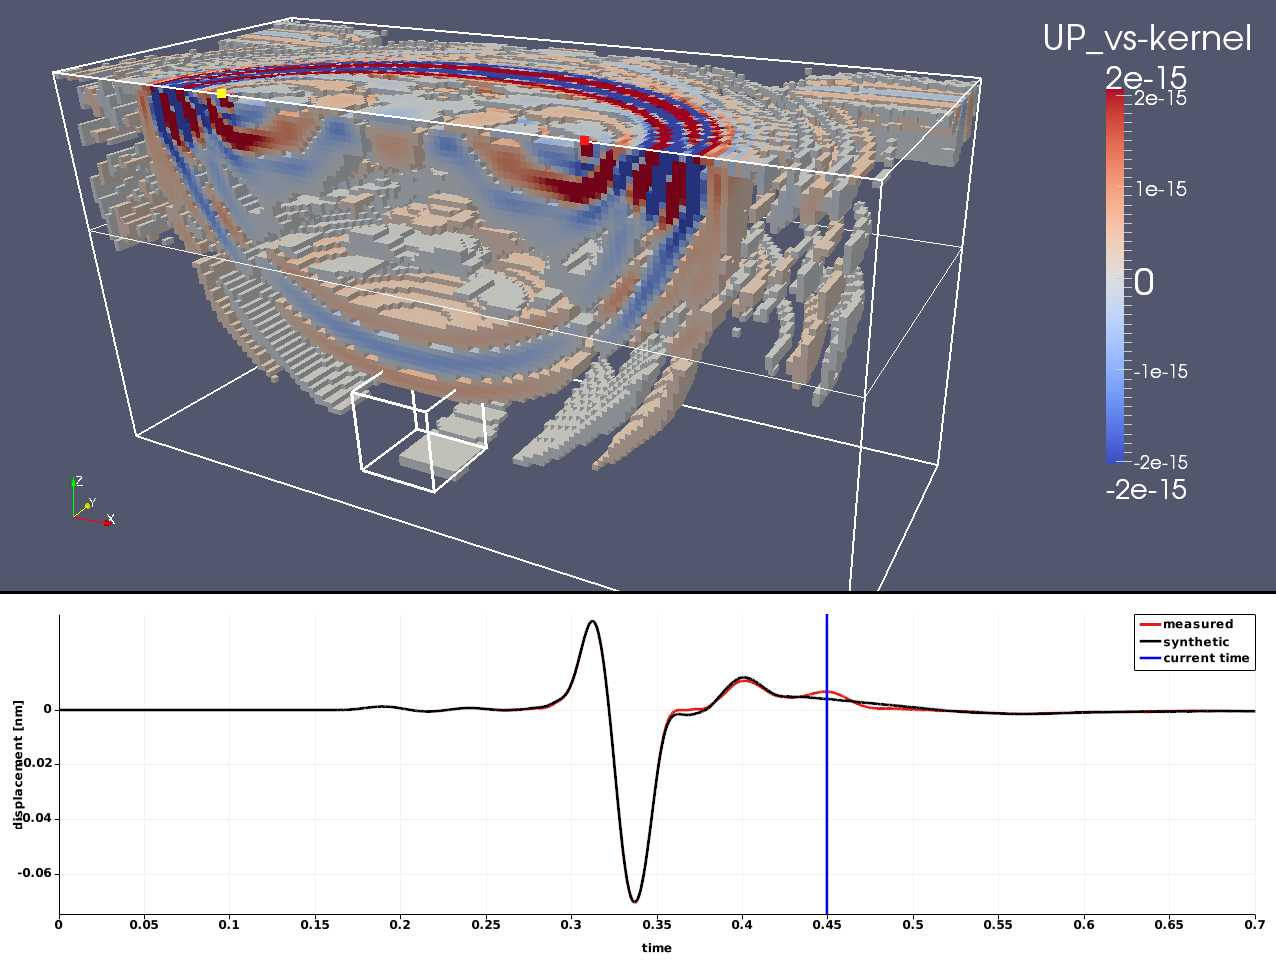
\includegraphics[width=\textwidth]{images/title_time_kernel_analysis.jpg}}
\end{center}

\end{titlepage}
% END individual titlepage
%#########


%
%
%-------------------------------
% LICENSE
Copyright \copyright {\myyear \today} Florian Schumacher.
Permission is granted to copy, distribute and/or modify this document
under the terms of the GNU Free Documentation License, Version 1.3
or any later version published by the Free Software Foundation;
with no Invariant Sections, no Front-Cover Texts, and no Back-Cover Texts.
A copy of the license is included in the section entitled ``GNU
Free Documentation License''.

\vspace{1cm}

If you use \ASKI{} for your own research, please cite one of our papers \cite{Schumacher16}, 
or \cite{Schumacher16b}, as appropriate:

F.\ Schumacher, W.\ Friederich and S.\ Lamara, \\
"A flexible, extendable, modular and 
computationally efficient approach to scattering-integral-based seismic full waveform 
inversion", \\
\emph{Geophysical Journal International}, (February, 2016) 204 (2): 1100-1119\\
\url{http://dx.doi.org/10.1093/gji/ggv505}

Schumacher F, Friederich W.\\
"ASKI: A modular toolbox for scattering-integral-based seismic full waveform 
inversion and sensitivity analysis utilizing external forward codes".\\
\emph{SoftwareX} 5 (2016) 252--259,\\
\url{http://dx.doi.org/10.1016/j.softx.2016.10.005}

\vspace{1em}

This documentation was written in the hope that it will be useful to the user,
but it \emph{cannot be assured} that it is accurate in every respect or complete in any sense.
In fact, at some places \emph{this manual is work in progress}.\\
Please do not hesitate to report any inconsistencies by
opening (or adding to) an "issues" topic on \url{https://github.com/seismology-RUB/ASKI}
or to improve this documentation by incorporating your experiences with \ASKI{} 
and your personal experience of getting used to it (at best by modifying the source and issuing a pull request
on gitHub, in any case let us know about it! Thanks).
When you have developed new \ASKI{} components or 
have modified existing once, please extend / modify the \ASKI{} documentation accoringly.

Furthermore, I am aware of the poor \LaTeX coding of this document (at the moment, \verb+\sloppy+ is used
at the beginning of the document to avoid overfull hboxes in many places). There is a lot of potential
to improve the document 
style, hence the readability of the manual as a whole, as well as the coding style of the 
particular \lcode{.tex} files. \emph{Please do not hesitate to improve!}

The \LaTeX source files and all related components of this document are available via
\url{https://github.com/seismology-RUB/ASKI}~, subdirectory \lcode{devel/doc/ASKI_developers_manual/}
of the repository.
\begin{flushright}
Florian Schumacher, \mydate \today
\end{flushright}

%% \newpage
%% %
%% %-------------------------------
%% % SECTION Introduction
%% %#############################################################
%% \section*{Guide Through This Manual}
%% %#############################################################
%% %
%% Bracketed comments starting with ``{\bf TODO IN THE FUTURE:}'' are intended to mark ideas for future work. 
%% So please ignore if you are just applying the code.
%
%-------------------------------
% TABLE OF CONTENTS
\newpage
\tableofcontents
\newpage

%-------------------------------
% SECTION how is the code documented in general
%#############################################################
\section{Introduction and guidelines for \ASKI{} developers} \label{sec:intro}
%#############################################################
%
The development of (what became) the software package \ASKI{} started in 2010 and from the beginning, auxilliary
Fortran modules were utilized (such as e.g.\ \lcode{errorMessage} and many more) which were developed by
Wolfgang Friederich (in many cases a lot earlier than 2010) and applied in the seismology group of Ruhr-University
Bochum (RUB) in a lot of different software projects (e.g.\ also in Gemini) via a separate ``include'' repository. 
As a result, \ASKI{} modules 
originating from this ``auxilliary software library'' most likely provide more functionality than \ASKI{} 
requires. After moving the \ASKI{} developers repository to \url{gitHub.com} in 2016, the \ASKI{} modules from 
``include'' were permanently forked from the RUB-internal code repository and may now be optimized
for used with \ASKI{} (not intended to merge them back into the original ``include'' repository at RUB, except
for bug-fixes and fundamental enhancement of general functionality). So, if you wonder why you come accross 
subroutines that are not used in \ASKI{} (so far!!), this might be a reason why.

\subsection*{Guidlines w.r.t.\ the \lcodetitle{git} repository}
At the moment, there are two branches on \lcodetitle{gitHub.com}: \lcode{master} and \lcode{develop}.

The \lcode{master} branch is intended to contain the latest stable version of the software package
(as also communicated in publications as well as the \ASKI{} user manual). \emph{No regular commits}
should be performed to the \lcode{master} branch, changes should only be merged from the \lcode{develop}
branch!

The \lcode{develop} branch is intended for development of new functionality (as its name says):
\begin{itemize}
\item The current state of the \lcode{develop} branch may be unstable or incomplete (e.g.\ in terms of documentation etc.).
\item \emph{Pull requests} should be issued to the \lcode{develop} branch only (and \emph{not} to the \lcode{master} branch)!
\item When a new portion of functionality is fully implemented and documented (thus, a ``stable'' state is reached), you may
  immediately merge the \lcode{develop} branch into the \lcode{master} branch. You don't need to wait until there is a new
  official ``version'' or something, you sould provide the latest stable version as quickly as possible to the user community.
\item On the \lcode{develop} branch, \emph{do not} commit \lcode{pdf}s of the \LaTeX{} documents (like the manuals, etc.) 
  each time you modify the documents! \emph{Only} before merging into the \lcode{master} branch commit a re-compiled \lcode{pdf}
  for each document (so that in the \lcode{master} branch the \LaTeX{} source corresponds to the repsective \lcode{pdf}).
\item Locally, you may use yet more branches for development (like ``feature'' branches etc.), but for now the sparsely manned 
development team does not consider it necessary to have these kinds of branches also available on \lcode{gitHub.com}.
\end{itemize}

\subsection*{How is the code documented in general?}
The code files are commented extensively. Furthermore, almost all Fortran modules, derived types, 
subroutines and functions are documented using doxygen syntax, even though doxygen output is not
really optimal for Fortran code. doxygen documentation can be produced using the doxygen config
file \lcode{doc/doxygen.conf}:
After installing doxygen (and possibly modifying file \lcode{doxygen.conf} according to your needs), 
you should be able to produce doxygen html and latex documents
executing \lcode{doxygen doxygen.conf} from path \lcode{doc/}, which should create subfolder \lcode{doc/doxygen_output} 
containing directories \lcode{html} and \lcode{latex}. For the html documentation, open
\lcode{doc/doxygen_output/html/index.html} by a webbrowser of your choice. For producing a latex pdf document, 
execute \lcode{make all} from \lcode{doc/doxygen_output/latex}, which should document 
\lcode{doc/doxygen_output/latex/refman.pdf}

\subsection*{Please preserve your experience!}
If you struggled with the existing \ASKI{} documentation (user manual, comments in code, doxygen, developers 
manual) because it was inconsistent, incomplete or simply wrong and you invested time to find out how it works, 
\emph{please let future generations of users and developers benefit from your gained knowledge!}
Everybody knows that documenting code and writing manuals consumes a lot of time, but correct documentation 
is essential for everyone using and developing software, and I'm sure you know that from your own experience.
So, please invest a bit more time in correcting/extending the \ASKI{} documentation
(where applicable: user manual, comments in code, doxygen, developers manual), otherwise your knowledge
is lost forever (you might even lose your knowledge yourself after some while, so please write it down!).

\emph{Thank you!} (on behalf of everybody)

%
%-------------------------------
% SECTION ASKI versioning
%#############################################################
\section{\ASKI{} versions}
%#############################################################
%
\ASKI{}'s release version numbering does not follow any standard of version numbering. 
Since releases were not very frequent so far and the source code was not publically available under version control, 
it was considered sufficient to have only a simple numbering for the purpose of distinguishing release versions.
In case that developments and releases become more frequent in the future, the \ASKI{} developers might consider
to follow some standard for future release version numbering.

\subsection*{\ASKI{} \lcodetitle{0.3}}
\ASKI{}'s first release version was numbered \lcode{0.3}, with \lcode{0} indicating a pre-release
that was not very well tested at that point and \lcode{3} being the third version of internal
development when porting from another internal versioning repository.

\subsection*{\ASKI{} \lcodetitle{1.0}}
After some while of intensive testing and application of \ASKI{} to synthetic and real-world cases, 
as well as development of a lot of \ASKI{} tools, version \lcode{1.0} was released as the first
ready-to-use version of \ASKI{}.

\subsection*{\ASKI{} \lcodetitle{1.1}}
In general, version \lcode{1.1} should be compatible with \lcode{1.0} in terms of file formats and general use
of the software. The main reason for this release was the fix of a pointer problem with \lcode{gfortran}.
Compared with the previous release, some more tools are available (\lcode{addSpikeCheckerToKim}, 
\lcode{createSpectralFilters}, \lcode{create_ASKI_evstat_filters.py}) and forward-code-specific 
definition of complex frequencies is available (e.g. for use with Gemini). Some bugs were fixed.

\subsection*{\ASKI{} \lcodetitle{1.2}}
Version \lcode{1.2} is just an intermediate version number and denotes the status of the code when moving the 
development repository permanently to git and providing the current working ready-to-use version of \ASKI{} by the 
master branch of repository \url{https://github.com/seismology-RUB/ASKI}.

Significant changes to version \lcode{1.1}:
\begin{itemize}
\item 
There is an additional subdirectory \lcode{devel/} containing developer tools and developer documentation.

\item
The source files of the \ASKI{} user manual as well as a compiled pdf of the manual are provided now in subdirectory
\lcode{doc/}

\item 
Inversion grids of type \lcode{chunksInversionGrid} now provide base cell refinement capabilities (at the moment
a random ``toy'' method is implmemented for illustration, but serious refinement method can now be implemented
easily into module \lcode{chunksInversionGrid}.

\item New/renamed/removed tools:

  \lcode{chunksInvgrid2vtk} for special vtk files related to chunks and refined cells 

  \lcode{createShoreLines} (Fortran executable) and \lcode{create_shore_lines.py} (Python program
  utilizing the \lcode{f2py} interface generator) for generating shore line vtk files from native binary GSHHS 
  shore line data files

  Executable \lcode{createMeasuredData} was renamed in \lcode{transformMeasuredData}

  Python script \lcode{create_ASKI_evstat_filters.py} is removed (functionality not required anymore)
\end{itemize}

\subsection*{The \lcodetitle{gitHub} master branch}
After porting \ASKI{} to \url{https://github.com/seismology-RUB/ASKI}, the current version of its master branch should
serve as a stable version to use, along with the current versions of the forward code packages supported by \ASKI{}.

%
%-------------------------------
% SECTION developers tools 
%#############################################################
\section{\ASKI tools for developers} \label{sec:devel_tools}
%#############################################################
%
%-------------------------------------
\subsection{\lcodetitle{adapt\_GPL\_headers.py}} \label{ssec-devel_tools:adapt_GPL_headers.py}
%-------------------------------------
Script \lcode{devel/adapt_GPL_headers.py} adapts GPL (and GFDL) headers of given files.
Executing \lcode{adapt_GPL_headers.py -h} will print a usage message.

For the \ASKI{} source files given as the positional arguments list (at least 1 must be
given), the license headers are adapted by year and/or \ASKI{} version, as specified by options
\lcode{-y, --year} and \lcode{-ver, --version}, respectively (at least one such option must be given, 
as otherwise there is nothing to do).

The program detects file headers of specific form, having the following properties:
\begin{itemize}
\item[] {\bf max length:} The headers are expected within the first \lcode{NLINE} lines of a file (default: 20)
\item[] {\bf start line:} The headers start at the first line containing the following characters (possibly 
  preceded by some commetary characters): 76 \lcode{-} characters.
\item[] {\bf end line:} The headers end by the first line after start line containing the following characters 
  (possibly preceded by some commetary characters): 76 \lcode{-} characters.
\item[] {\bf text segment:} there must be at least one line (between start and end line) that contains one of the
  following text samples:
  \begin{itemize}
  \item[] \lcode{under the terms of the GNU General Public License}
  \item[] \lcode{under the terms of the GNU Free Documentation License}
  \end{itemize}
\item[] {\bf assumption:} first line after start line does \emph{not} contain ``ASKI version~`` (if so, it is ignored)
      but contains ``Copyright~'' followed by the year (year = the word following the \emph{first} occurence of 
      ``Copyright~'' in that line). The year will be replaced by a new value (if \lcode{-y, --year} is indicated).
      If in the original header, the year ends a sentence, i.e.\ ends on a period ``.'', this period
      will be preserved. \emph{Nowhere else in the header will the year be searched for and adapted!}
\end{itemize}

%- - - - - - - - - - - - - - - - - - - - - - - - - - - - -
\subsubsection{Options}
%- - - - - - - - - - - - - - - - - - - - - - - - - - - - -
\paragraph{\lcode{-h, --help}}
print usage message
%- - - - - - - - - - - - - - - - - - - - - - - - - - - - -
\paragraph{\lcode{-y YEAR, --year YEAR}}
If set, then the copyright year (i.e.\ the word following the first occurence of ``Copyright~`` in the 
first line of the header text body) will be set to the given value \lcode{YEAR} (character string, not 
checked if it is a number).
%- - - - - - - - - - - - - - - - - - - - - - - - - - - - -
\paragraph{\lcode{-ver VERSION, --version VERSION}}
If set, then the \ASKI{} version will be set to the given value \lcode{VERSION}
(character string, not checked if it contains numbers). Give the version here
by numbers only, e.g. \lcode{1.3} for \ASKI{} version 1.3
%- - - - - - - - - - - - - - - - - - - - - - - - - - - - -
\paragraph{\lcode{-n NLINES, --nlines NLINES}}
Optional: if set, then the header is expected to be contained within
the first \lcode{NLINE} lines of each indicated file (if not set, default value of 20 is used).

%- - - - - - - - - - - - - - - - - - - - - - - - - - - - -
\subsubsection{Positional arguments}
%- - - - - - - - - - - - - - - - - - - - - - - - - - - - -
\paragraph{\lcode{ASKI_src_files ...}}
List of filenames (relative or absolute) indicating all files for which the header should be adapted.
You may as well use regular expressions on the command line such as\\
\lcode{f90/* py/* doc/ASKI_manual/*.tex devel/* devel/*/*}\\
The program generates warnings if particular files cannot be adapted (because there is no header found
as expected) and continues to process the rest of the files. 

%-------------------------------------
\subsection{\lcodetitle{create\_Makefile\_rule.py}} \label{ssec-devel_tools:create_Makefile_rule.py}
%-------------------------------------
Calling\\
\lcode{devel/create_Makefile_rule.py newTool}\\
from the \ASKI{} installation directory will print a complete Makefile rule for target \lcode{newTool}
to screen (output should be re-directed into a file by something like \lcode{> output.txt}).
Any required libraries (\lcode{BLAS}, \lcode{LAPACK} etc.) should be accounted for correctly.
Otherwise you should update script \lcode{create_makefile_rule.py}, in particular routine 
\lcode{required_libs_for_depobs}: please add any library requirements for new/modified modules that you have
developed.

%-------------------------------------
\subsection{\lcodetitle{create\_rules\_mk.py}} \label{ssec-devel_tools:create_rules_mk.py}
Script \lcode{create_rules_mk.py} (contained in \lcode{devel/}) can be utilized to re-create file 
\lcode{rules.mk}. From the \ASKI{} installation directory, call\\
\lcode{devel/create_rules_mk.py > rules.mk}\\
(you might want to backup the existing \lcode{rules.mk} before you overwrite it, just in case).


%
%-------------------------------
% SECTION extend to new forward code
%#############################################################
\section{Add support for another external forward code} \label{sec:extend_forward_code}
%#############################################################
%
\ASKI{} does not implement an intrinsic code for simulation of seismic wave propagation in order to 
solve the forward problem, but instead provides generalized interfaces to different external wave 
propagation codes. At the moment, the 1D semi-analytical code Gemini \cite{friederich_wd1995} and the 3D spectral 
element code SPECFEM3D \cite{TrKoLi08} are supported in \emph{both}, Cartesian and spherical framework. 
Additionally \ASKI{} supports the 3D nodal discontinuous Galerkin code NEXD \cite{Lambrecht.2015}
and we plan to implement support for the Finite Difference code SOFI \cite{bohlen2002parallel}
in the future. 

Here is a conceptual recipe describing the steps that need to be done to add another forward code to the 
ASKI software package:

%-------------------------------------
\subsection{What functionality / information must the forward code provide / produce for use with \ASKI{}?} \label{ssec-extend:forward_output}
%-------------------------------------
The forward code must be able to provide information/definitions of the quantities listed in the following. 
Therefore, the forward code most likely need to be extended / modified for use with \ASKI{}. However, the forward 
code is absolutely free in the way it provides this information, i.e.\ any standard (parameter) files can be
used to provide information (the code is not to be modified in this case) or any files of some own file format 
can be produced (even parallel output can used, provided the knowledge of how to read it/locate the files), 
or any assumptions can be made on the quantities (assumptions on filenames, (sub)grids, model
structure (e.g.\ 1D), etc.). Information on the following quantities just needs to exist somehow (either by
standard functionality of the program, by assumptions or by files of arbitrary (new) format. How this information
is communicated to \ASKI{} is explained below in sec.~\ref{ssec-extend:ASKI_interface}.

\subsubsection{forward grid}
The forward code must provide point coordinates of the grid on which it produces
wavefield output (see below displacements / Green functions). For grid-based forward codes, it is efficient 
(thus recommended) to use a (sub)grid of the simulation grid. An independent point grid can be chosen just as well, 
but this requires additional interpolation of wavefields (and, thus, additional costs). For modal methods (that
do not have a simulation point grid), a suitable point grid must be chosen on which the wavefields are evaluated.

In \ASKI{}, these forward grid points (on which the wavefields are provided) are referred to as \emph{wavefield points}
and they are completely independent of the chosen inversion grid, except that they should be contained in the
inversion grid cells and they cover the domain sufficiently dense such that each inversion grid cell contains
enough wavefield points (``enough'' depends on the method of pre-integration).

\subsubsection{elastic model on wavefield points}
The forward code must provide model values on the wavefield points in the model prametrization as chosen in 
the \ASKI{} main paramter file (at the moment only elastic parametrizations, see user manual, chapter ``Files'', 
section on main parameter file), e.g.\ if model parametrization \lcode{isoLameSI} is chosen, values of 
isotropic Lam\'e paramters and densitiy in SI units must be available.

In \ASKI{}, these model values are referred to as \emph{kernel reference model}.

\subsubsection{spectral displacement wavefield propagating from seismic sources into medium as well as its strains}
On the wavefield points, the forward code must provide values of spectral displacement excited by each of the seismic 
sources involved in an inversion. The displpacement components (direction of particle movement) must be provided 
in directions of global Cartesian coordinates (even for spherical media). Otherwise the implemented kernel formulae 
do not work. For time-domain forward methods, the forward code must be extended by an
on-the-fly Fourier transform in order to provide this quantity (transformation of the wavefields to 
frequency domain \emph{after} the complete simulation i.e.\ not on-the-fly is of course also possible, but in 
case of SPECFEM was considered unsuitable due to huge memory requirements, also refer to \myref{ssec-extend:Goertzel}).

In the same way, \ASKI{} requires strains on the wavefield points, i.e.\ quantities
\[
\frac{1}{2}\left(\frac{\partial u_k}{\partial x_\ell} + \frac{\partial u_\ell}{\partial x_k}\right)
\]
for all global Cartesian directions $k$ and $\ell$, where $u$ denotes particle displacement.

In \ASKI{}, these spectral displacment and strain values are referred to as \emph{kernel displacement}.

\subsubsection{spectral synthetic data in format required by \ASKI{}} \label{subsub:synthetic_data}
Essentially the same values as for kernel displacement, but evaluated at the receiver positions 
in directions of the used station components (by which the measured data is provided, see user manual chapter
``Basic steps'', section on data in \ASKI{}). Also these values must be provided in the file format of synthetic
data (see user manual, chapter ``Files'', section on synthetic data files).

In the future, it would be better to have a set of interface modules for synthetic data (just as
for wavefield points, kernel reference model, kernel displacement, kernel Green tensor \myaref{ssec-todo:new})

\subsubsection{spectral Green's functions originating at receiver positions as well as its strains}
``Green's functions originating at receiver positions'' here means the spectral displacement field 
(on wavefiled points) excited by a
unit point force at the receiver position (pointing into the direction of a particular station component, i.e.\
there is such a Green's function for each station component) using an impulsive source-time function (Dirac-delta
impulse). For time-domain forward methods that need to use an approximation to the Dirac-delta impulse (e.g.\ a
very thin Gaussian source-time-function), it is highly recommended to deconvolve it from the resulting wavefield:
In case of SPECFEM this was found out to be necessary, because the inversion process fitted phase-shifted 
seismograms when just using a thin Gaussian. Moreover (just as for kernel displacements), in time-domain
forward methods an on-the-fly Fourier transform must be applied to produce spectral output 
\myaref{ssec-extend:Goertzel}

In the same way, \ASKI{} requires the strains of Green's functions on the wavefield points, i.e.\ quantities
\[
\frac{1}{2}\left(\frac{\partial g_k}{\partial x_\ell} + \frac{\partial g_\ell}{\partial x_k}\right)
\]
for all global Cartesian directions $k$ and $\ell$, where $g$ denotes the particle displacement of a particular
Green's function.

In \ASKI{}, these spectral displacment and strain values are referred to as \emph{kernel Green tensor}.

\subsubsection{some script running all simulations in a FWI iteration}
For iterative FWI with \ASKI{}, in each iteration the kernel displacement wavefields must be produced for each
event in the event list and kernel Green tensor wavefields must be produced for each station in the station list
at each station component involved in the inverted data set. In order to conduct all required simulations 
conveniently (and consistently!), it is highly recommended to have some kind of script that gets information
from \ASKI{} parameter files (about event, station locations, paths where to write the file output etc), 
sets all required parameter files of the forward code and conducts the simulation (by issuing a system call
or something). For SPECFEM this is done by a (huge) python script 
\lcode{run_specfem3d(Globe/Cartesian)ForASKI_simulations.py}


%-------------------------------------
\subsection{Make \ASKI{} understand the forward code: \ASKI{} interface sub-modules} \label{ssec-extend:ASKI_interface}
%-------------------------------------
In order to make \ASKI{} understand a new forward code, several things have to be extended / modified in \ASKI{}'s 
source code. First of all, a forward code is denoted by a character string (without spaces) that is read from 
key \lcode{FORWARD_METHOD} of the main parameter file. All modules and routines for which any action depends on the
forward code will check the value of this character string. 

In function \lcode{validTypeInversionGrid} of module \lcode{inversionGrid}, it should be implemented whether
the new forward method is incompatible with some inversion grids (e.g.\ Cartesian methods should be incompatible
with spherical inversion grids and vice verca) or integration weight types (e.g.\ ``external'' integration weights,
type 6, are only supported by special methods).

In functions \lcode{methodHasComplexKernelFrequency} and \lcode{getComplexKernelFrequency} of module 
\lcode{complexKernelFrequency}, please define whether the new forward code uses complex frequencies
(such as Gemini) and define how they compute from frequency index and frequency step. 

Furthermore, for all modules \lcode{wavefieldPoints}, \lcode{kernelReferenceModel},
\lcode{kernelDisplacement},
\lcode{kernelGreenTensor} the following steps need to be done, \emph{exemplarily} described here for 
\lcode{kernelDisplacement} and new forward code name NEWCODE
\begin{enumerate}
\item Carefully study the functionality of module \lcode{kernelDisplacement} in terms of what routines can
  be called from outside and what they provide (e.g.\ strains and displacement fields are provided on all wavefield 
  points for one frequency that was read in before by \lcode{readFrequencyKernelDisplacement}).
  It is helpful to compare the submodules of existing forward methods (e.g. \lcode{specfem3dKernelDisplacement}).
  This way, you should find out how a submodule \lcode{newcodeKernelDisplacement} for code NEWCODE could be 
  organized best and it can even give you a hint how method NEWCODE could best provide any file output that is to
  be newly implemented.
\item Create the new module \lcode{newcodeKernelDisplacement} (can be of different name, could be more than one
  module, but please keep it simple!):
  \begin{enumerate}
  \item Declare derived type \lcode{newcode_kernel_displacement} defining the kernel displacement object of the new 
    forward method (e.g.\ arrays and scalars for values and meta data required to manage the wavefield output
    provided by the forward code).
  \item For each function or subroutine in module \lcode{kernelDisplacement} that forks to a particular 
    forward method, implement a realization for your new module (either as a full routine in module 
    \lcode{newcode_kernel_displacement} or as a short piece of code in the if-statements of module 
    \lcode{kernelDisplacement} if the respective feature is not supported or has a trivial/general implementation).
    This assures that the new forward code is allowed to define its own file formats or to re-use standard 
    (parameter)files (providing here the knowledge of how to access these files or any required information).
    \emph{Make sure} that the respective routine in \lcode{kernelDisplacement} works correctly when it is called, 
      refer to the (doxygen) commentary of the \lcode{kernelDisplacement} routine: e.g.\ usually only pointers to 
      values are passed to module \lcode{kernelDisplacement} and deallcation has to be done 
  \end{enumerate}
\item Add the new forward method to module \lcode{kernelDisplacement}:
  \begin{enumerate}
  \item Use the module by \lcode{use newcodeKernelDisplacement}.
  \item For each function or subroutine in module \lcode{kernelDisplacement} that forks to a particular 
    forward method, add an \lcode{else if} branch and call the respective routine in module 
    \lcode{newcodeKernelDisplacement} (or implement trivial solution directly).
  \end{enumerate}
\item Update \lcode{rules.mk}:
  If module \lcode{newcodeKernelDisplacement} uses modules \lcode{module1}, \lcode{module2}, \lcode{module3} (etc.)
  add a new line of form \\
  \lcode{newcodeKernelDisplacement.o: module1.o module2.o module3.o}\\
  Otherwise, \lcode{rules.mk} does not need to be modified.
  Alternatively, use \lcode{create_rules_mk.py} \myaref{ssec-devel_tools:create_rules_mk.py}
\item Update \lcode{Makefile}: Every rule (to compile an \ASKI{} executable) that depends on 
  \lcode{kernelDisplacement.o} must now additionally depend on \lcode{newcodeKernelDisplacement.o}~.
  As an alternative to expanding the rules manually, you may utilize script \lcode{py/create_Makefile_rule.py}
  \myaref{ssec-devel_tools:create_Makefile_rule.py}
\end{enumerate}

%-------------------------------------
\subsection{Import updated model to the forward code for next iteration of FWI} \label{ssec-extend:forward_import}
%-------------------------------------
In order to do iterative FWI with \ASKI{}, the model derived in an iteration of FWI must be used as background 
Earth model for the next iteration of FWI. Hence, it must be transferred back into the forward solver. 
This process can be very different, dependent on the type of forward method (modal method or grid-based) and 
dependent on whether only a sub grid was used as wavefield points for \ASKI{} and whether the simulation domain
of the forward code exceeds the \ASKI{} inversion domain.

\ASKI{} handles inverted Earth models (model updates as well as new model values) by different files that are
not self-consistent (values in \lcode{.kim} files correspond to inversion grid cells, which themselves are defined
elsewhere, namely in an individual way by the respective inversion grid sub module). This storage of information
is intended for internal \ASKI{} use only. Therefore, \ASKI{} offers to export such inverted models in a 
self-consistent format that may be used by the individual fortward code to communicate the model information
(\ASKI{} executable \lcode{exportKim}, option \lcode{-otxt}, see \ASKI{} user manual). The resulting text file
contains coordinates of inversion grid cell centers as well as the model values which are assigned to these points.
The cell centers act as some kind of unstructured grid of control nodes on which the model values are given.
Furthermore, information about neighbouring cells (i.e.\ neighbouring control nodes) as well as approximate average
spatial extend of the inversion grid cells (i.e.\ the influence radius of the control nodes) are given in the file.
The \ASKI{} user manual dedicates a section in chapter ``Files'' to the exact format of this text file.

Since in \ASKI{} the forward and inversion grid are in general independent of each other (and forward codes do not
even need to be grid-based), you will require an individual transference of \ASKI{} inverted models to the model 
description of the new forward code. Modal methods will have to approximate expansion coefficients from the model
values on the control nodes (inversion grid cell centers) and grid-based forward codes using structured grids may 
realize much simpler interpolation methods than those using unstructured grids. E.g.\ for the \lcode{SPECFEM} and
\lcode{NEXD} forward methods, an unstructured 3D interpolation after Shepard \cite{Shepard68} was implemented, 
which is founded on inverse-distance weighting and accounts for issues of nearby points, direction and slope. 
For sure, the current implementation of subroutine \lcode{shepard_interpolation_model_ASKI} in module 
\lcode{model_ASKI} of the \lcode{SPECFEM3D_Cartesian_for_ASKI} extension package (file \lcode{model_external_values.f90})
can be improved w.r.t.\ computational performance, but it may well serve you as an illustration how to implement
Shepard's agorithm. 

%-------------------------------------
\subsection{As an option: use forward-code-specific quadrature rules for kernel pre-integration} \label{ssec-extend:external_intw}
%-------------------------------------
Using integration weights of type 6 (``external integration weights'') is only supported along with a suitable 
type of inversion grid, at the moment only \lcode{specfem3dInversionGrid}. This type of integration weights
is potentially useful for element-based (weak-form) forward methods: Their own quadrature rules for integration onto 
their elements may be re-used by \ASKI{} for kernel pre-integration. Also this may be beneficial for special kinds of 
forward grids in combination with specific inversion grids, where you have certain pre-knowledge of how to 
integrate over the cells with high precision. 

In order to realize the use of these special kinds of integration rules, the inversion grid module needs to provide the
integration weights: routine \lcode{transformToStandardCellInversionGrid} must be called with 
\lcode{type_standard_cell} equal to $-1$ on input in order to request the inversion grid to return full 
integration weights instead of jacobian values in return variable \lcode{jacobian}.
Hence, this is only possible for specific types of inversion grids that support this input value (at the moment 
only \lcode{specfem3dInversionGrid}). So you might need to add another inversion grid type to \ASKI{} that works 
with your forward code (see sec.~\ref{ssec-invgrid:external}{}) or modify an existing inversion grid submodule 
accordingly. In particular, routine \lcode{validTypeInversionGrid} must accept the use of type 6 integration 
weights along with your inversion grid type.

%-------------------------------------
\subsection{Time-domain forward methods: Choosing a method of on-the-fly Fourier transform} \label{ssec-extend:Goertzel}
%-------------------------------------
For time-domain forward methods, the spectral wavefields need to be produced by Fourier transform from the 
time-domain wavefield \emph{at every wavefield point}. Doing this by the fast Fourier algorithm (FFT) has several
issues/drawbacks:
\begin{itemize}
\item since the time-series will be heavily oversampled (due to Courant stability criteria), the frequency-domain 
  spectra will be oversampled, too (you compute more than you actually need, usually you require output at very 
  few frequencies only)
\item the frequency discretization of the output spectra is pre-defined by the time sampling of the time series
  and cannot be chosen independently (as requested by the \ASKI{} user and defined in the \ASKI{} main/iter parameter 
  files)
\item for realistic applications, you usually cannot hold the complete wavefield (at all wavefield points) in 
  memory until you can apply the FFT at the very end of the simulation (for FFT you need to have the complete 
  time series available)
\end{itemize}
In order to evaluate the Fourier transform of the waveifields at the particular set of requested frequencies 
$f_k = \omega_k/2\pi$, $k = 1,N_F$, the sums
\begin{align}
S(\omega_k) = S_k = \Delta t \sum_{j=1}^{N_T} s(t_j) \, e^{-i\omega_k t_j} = \Delta t \Big[ \sum_{j=1}^{N_T} s(t_j)\cos(-\omega_k t_j)\;+\; i\, \sum_{j=1}^{N_T} s(t_j)\sin(-\omega_k t_j) \Big] \quad, \label{eq:inversion_implement_DFT}
\end{align}
have to be computed for each $k$, where the $s(t_j)$ represent samples of displacement (or strain) components at 
one location of a wavefield point (or the receiver position in case of producing spectral synthetic data as
described in \myref{subsub:synthetic_data}). Note that eq.~\eqref{eq:inversion_implement_DFT} is a time-discretized
simple approximation of the Fourier transform of the continuous signal $s(t)$:
\begin{align}
  S(\omega) = \mathcal{F}[s(t)](\omega) = \int_{-\infty}^{\infty} s(t) \, e^{-i\omega t}\, \mathrm{d}t \;.
\end{align}
In discretized setting, time $t_j$ is represeted as $(j-1)\Delta t$ (time starts at $t_1=0$) and angular frequency 
$\omega_k$ as $2\pi f_k = 2\pi \ell_k \Delta f$, where $\ell_k$ is the $k$\textsuperscript{th} \ASKI{} 
frequency index (normally denoted as \lcode{jf} or so, here $j$ is already used so please excuse this different
notation $\ell$ here).

A straight-forward way of evaluating the left-hand-side representation of \eqref{eq:inversion_implement_DFT} 
on the fly (i.e.\ \emph{without} 
having all samples $s(t_j)$ simultaneously available but only the latest sample at a time) would be to add summand
$s(t_j) \, e^{-i\omega_k t_j}$ to a complex-valued variable $S_k$ (initialized by $0$) in iteration $j$ of the
forward simulation. This requires (in each iteration of the time loop, for each wavefield/strain component, 
for each wavefield point and for each frequency) $2$ real-valued multiplications (multiplying the complex number 
$e^{-i\omega_k t_j}$ by the real number $s(t_j)$ and two real-valued additions (adding the complex number 
$s(t_j) \, e^{-i\omega_k t_j}$ to the current complex value in $S_k$). Note that the right-hand-side form of
\eqref{eq:inversion_implement_DFT} has the very same requirements.
Multiplying the resulting $S_k$ by $\Delta t$
at the very end (or incorporating $\Delta t$ in pre-computed constants $e^{-i\omega_k t_j}\,\Delta t$, 
$\cos(-\omega_k t_j)\,\Delta t$ or $\sin(-\omega_k t_j)\,\Delta t$ that are computed
once before the time loop) is neglected in this argumentation of performance.

A computationally more efficient way of computing sum~\eqref{eq:inversion_implement_DFT} on the fly
is to apply an algorithm first described by Gerald Goertzel in 1958 \cite{Goertzel58} which for given $x$ computes
sums of the form
\[
\sum_{j=0}^{N} a_j\cos(j\,x)\quad\text{and}\quad \sum_{j=1}^{N} a_j\sin(j\,x)
\]
and can be adapted here to compute $S_k$ by the righ-hand side of~\eqref{eq:inversion_implement_DFT} choosing 
$x = -\omega_k\,\Delta t$ and $a_j = s(t_j)$:
\begin{align}
  W_r &= 2\cos(x) \label{alg:goertzel_1}\\
  W_i &= \sin(x) \label{alg:goertzel_2}\\
  U_1 &= 0 \\
  U_2 &= 0 \\[1.5ex]
  &\text{for $j=N_T,\dots 2$ do:}\label{alg_goertzel_5}\\
  U_0 &= s(t_j) + W_r \, U_1 - U_2\label{alg_goertzel_6}\\
  U_2 &= U_1\\
  U_1 &= U_0 \label{alg_goertzel_8}\\[1.5ex]
  &\text{after iterating (backwards in time) down to $t_2$, the  spectral value $S_k$ computes as:}\notag\\
  \mathfrak{Re}(S_k) &= \Delta t\,\left(s(t_1) + 0.5\,W_r \, U_1 - U_2\right)\label{alg_goertzel_10}\\
  \mathfrak{Im}(S_k) &= \Delta t\,W_i \, U_1
\end{align}
In each iteration of the time loop (i.e.\ lines~\eqref{alg_goertzel_6} to \eqref{alg_goertzel_8}), 
for each wavefield/strain component, 
for each wavefield point and for each frequency here only $1$ real-valued multiplication is required
(in line~\eqref{alg_goertzel_6}) and also two real-valued additions (in the same line). Compared with the 
explicit summation described above, we save one multiplication here. This sounds not so much, but
since a real-valued multiplication is usually much more expensive than a real-valued summation, this algorithm
may be close to twice as fast as the explicit summation above. 

The problem of the algorithm in this form, however, is that it requires \emph{reverse} knowledge of the imput
time series $s(t_j)$, first requiring the value at last time and iterating backwards in time. This, of course,
does not allow to do an on-the-fly Fourier transform in simulations of seismic waves (propagating \emph{forward}
in time).

Looking at the proof of the algorithm as given in \cite{Goertzel58}, I (Florian Schumacher, Sep 2016) tried to 
find an analogous recursion relation that allows to step through the time series in \emph{forward} direction
from $s(t_1)$ up to last sample $s(t_{N_T})$) but was not successful. However, there is a trivial way to adapt the
above algorithm for our purposes, making use of properties of the Fourier transform: Inserting the time
series $s(t_j)$ into the algorithm in \emph{forward} order (starting with $s(t_1)$, $s(t_2)$ \dots) means 
mathematically to compute the Fourier transform of $s(-t)$. This can be compensated by negating the frequency,
i.e.\ choosing $-\omega_k$ instead of $\omega_k$ everywhere, due to the time-reversal property of the Fourier transform:
\[
\mathcal{F}[s(-t)] = S(-\omega)
\]
However, this only fixes the time-reversal of the time series. Since Goertzel's algorithm assumes the last sample 
of the time to come first, technically the time series is assumed to start at time $-T = -(N_T-1)\Delta t$ and
to end at time $0$. Therefore, additionally to negating the frequency, we need to compensate for a time shift
(resulting in a constant phase shift of the output spectrum) applying the time-shift property of the Fourier transform:
\[
\mathcal{F}[s(t-T)] = S(\omega)e^{i\omega\,(-T)}
\]

Taking all considerations into account, we need to adapt the above original algorithm by Goertzel for our 
purposes in the following way:
\begin{itemize}
\item Choose $x = +\omega_k\,\Delta t$
\item Step forward through the time series, i.e.\ modify line~\eqref{alg_goertzel_5} as
  \hypersetup{draft=true}
  \begin{equation}
    \text{for $j=1,\dots (N_T-1)$ do:} \tag{\ref*{alg_goertzel_5}-b} %\label{alg_goertzel_5b}
  \end{equation}
  \hypersetup{draft=false}
\item Correct the computation of the real part of the spectral value by modifying line~\eqref{alg_goertzel_10} as
  \hypersetup{draft=true}
  \begin{equation}
    \mathfrak{Re}(S_k) = \Delta t\,\left(s(t_{N_T}) + 0.5\,W_r \, U_1 - U_2\right) \tag{\ref*{alg_goertzel_10}-b} %\label{alg_goertzel_10b}
  \end{equation}
  \hypersetup{draft=false}
\item After the algorithm is completed, additionally correct for the time shift by
  \begin{equation}
    S_k = S_k \,e^{-\omega_k(N_T-1)\Delta t}
  \end{equation}
\end{itemize}

Demonstrating the significant performance improvement when using Goertzel's algorithm, compared with the
explicit summation, these two algorithms were implemented in the example
program \lcode{goertzel.f90}, provided in directory \lcode{devel/Goertzel/} of the \ASKI{} repository. Please 
refer to \lcode{devel/Goertzel/README.md} on any information regarding this example program, in particular 
on how to compile and run it.
\emph{Please note}, however, that e.g.\ in case of forward code \lcode{SPECFEM3D_Cartesian}, the overall
performance improvement of using Goertzel's algorithm (compared with explicit summation) is \emph{not}
noticeable, since these operations comprise only a part of the additional costs for producing output for \ASKI{}
and other things like array/memory access etc.\ also play an important role w.r.t.\ overall performance.


%-------------------------------
% SECTION new executable
%#############################################################
\section{Create new executables of the \ASKI{} toolbox based on its software library} \label{sec:executables}
%#############################################################
%
New Fortran executables can be created using existing \ASKI{} Fortran modules (or creating new ones, of course). 
A list of all \ASKI{} Fortran modules along with short descriptions about what functionality they provide, is
provided by the doxygen documentation (chapter 1 in the LaTex document and ``Modules'' (\lcode{namespaces.html})
in the html document).
In order to make life easier for all \ASKI{} users, the command line behaviour should be very similar to all
other Fortran executables of \ASKI{} (i.e.\ using module \lcode{argumentParser} and printing usage message
if some input is incorrect and, if required, setting \lcode{main_parfile} as last positional argument).

In order to correctly compile the new executable, here having exemplary name \lcode{newTool}, you need to:
\begin{enumerate}
\item Update \lcode{rules.mk}:
  If program \lcode{newTool} uses modules \lcode{module1}, \lcode{module2}, \lcode{module3} (etc.)
  add a new line of form\\
  \lcode{newTool.o: module1.o module2.o module3g.o}\\
  If any of the modules, e.g.\ \lcode{module2} was newly created and
  itself depends on other modules, e.g.\ \lcode{module4}, \lcode{module5},
  add a new line of form\\
  \lcode{module2.o: module4.o module5.o}

  If \lcode{newTool} does not use any modules and is not dependent on other files, \lcode{rules.mk} does not need 
  to be modified. 

  As an alternative to modifying \lcode{rules.mk} manulally (especially when extending existing modules that are
  used in many other modules), you can ultilize \lcode{create_rules_mk.py}
  \myaref{ssec-devel_tools:create_rules_mk.py}

\item Add a new rule for \lcode{newTool} to \lcode{Makefile}: 
  \begin{enumerate}
  \item Run script\\
    \lcode{devel/create_Makefile_rule.py newTool > rule.txt}\\
    from the \ASKI{} installation directory \myaref{ssec-devel_tools:create_Makefile_rule.py}
  \item Add content of \lcode{rule.txt} to \lcode{Makefile} (GNU-Make rule to compile executable \lcode{newTool}).
    The required libraries (\lcode{BLAS}, \lcode{LAPACK} etc.) should have been accounted for correctly
    (otherwise you should update script \lcode{create_makefile_rule.py}, in particular routine 
    \lcode{required_libs_for_depobs}; please add any library requirements for \lcode{newTool}).
  \item All general \ASKI{} executables from which all \ASKI{} users benefit, should be part of the rule of
    target \lcode{all}, so please add \lcode{newTool} there unless \lcode{newTool} is a very special executable
    that should be compiled explicitely by experienced users only (then, please stress this in the documentation).
  \end{enumerate}
\end{enumerate}


%-------------------------------
% SECTION inversion grid
%#############################################################
\section{Inversion grids} \label{sec:inversion_grid}
%#############################################################
%-------------------------------------
\subsection{Add another type of inversion grid} \label{ssec-invgrid:new-type}
%-------------------------------------
\begin{enumerate}
\item Create a new module (here using exemplary name \lcode{newInversionGrid}):
  \begin{enumerate}
  \item Declare derived type \lcode{new_inversion_grid} defining the new inversion grid.
  \item For each function or subroutine in module \lcode{inversionGrid} implement a realization for
    inversion grids of type \lcode{new_inversion_grid} (either as a full routine in module \lcode{newInversionGrid}
    or as a short piece of code in \lcode{select} statements of module \lcode{inversionGrid} if the respective feature is not
    supported or has a trivial/general implementation).
  \end{enumerate}
\item Add the new inversion grid type (here using exemplary name \lcode{newInversionGrid}) to module
  \lcode{inversionGrid}:
  \begin{enumerate}
  \item Use the module by \lcode{use newInversionGrid}.
  \item Increase \lcode{character_length_type_inversion_grid} if necessary.
  \item Extend string \lcode{all_valid_types_inversion_grid}.
  \item Add pointer of type \lcode{new_inversion_grid} to derived type \lcode{inversion_grid}.
  \item For each function or subroutine, add a \lcode{case} in the \lcode{select} clauses and call the 
    inversion-grid-specific routine (or implement trivial solution).
  \end{enumerate}
\item Update \lcode{rules.mk}:
  If module \lcode{newInversionGrid} uses modules \lcode{module1}, \lcode{module2}, \lcode{module3} (etc.)
  add a new line of form \\
  \lcode{newInversionGrid.o: module1.o module2.o module3.o}\\
  Otherwise, add a new line of the form\\
  \lcode{newInversionGrid.o:}
\item Update \lcode{Makefile}: Every rule (to compile an \ASKI{} executable) that depends on 
  \lcode{inversionGrid.o} must now additionally depend on \lcode{newInversionGrid.o}
\end{enumerate}

%-------------------------------------
\subsection{Using element grid of element-based forward method as inversion grid} \label{ssec-invgrid:external}
%-------------------------------------
%
For element-based forward methods (such as e.g.\ SPECFEM3D), it can be beneficial to use the volumetric elements
as inversion grid cells along with using the contained forward grid points as wavefield points: The localization
of wavefield points inside the inversion grid cells is known in this case and, optionally, also quadrature rules 
for numerical integration can be either known or should be computable (semi-)analytically.
If you would like to add this kind of functionality for your own newly added element-based forward method, you
are advised to have a close look at the realization of module \lcode{specfem3dInversionGrid}.

By SPECFEM3D, for instance, all forward grid points in a certain spatial subdomain are stored element-wise in a 
known order in some file, so that it is possible for module \lcode{specfem3dInversionGrid} to extract the 8 
corner points of the spectral elements from that set of coordinates (which are required for the 8-corner hexahedral 
vtk cell output) and to trivially locate the wavefield points inside the elements (and give their position
inside the hexahedral reference element $[-1,1]\times[-1,1]\times[-1,1] \subset \mathbb{R}^3$).

As an optional feature, the module \lcode{specfem3dInversionGrid} can provide the integration weights for 
numerical integration of the kernels on the spectral element that are also used by the spectral element method.
These have a high numerical accuracy due to the special distribution of points inside the element (GLL points).
In this case \ASKI{} can benefit from this knowledge and does not need to compute its own integration weights.
Alternatively, other types of \ASKI{} integration rules can be used along with an inversion grid of type 
\lcode{specfem3dInversionGrid}.

%
%-------------------------------------
\subsection{\lcodetitle{chunksInversionGrid}: implement a method of cell refinement} \label{ssec-invgrid:chunks-cell-ref}
%-------------------------------------
First, you should make yourself familiar with module \lcode{chunksInversionGrid}. Unfortunately, this module has
kept growing and became some kind of monsterous construct. There is definitely a lot of commentary in the
code, which mostly is formatted using doxygen syntax (regarding routines and variables descriptions), so it
might be worth referring to the doxygen documentation.
Additionally, fig.~\ref{ssec-invgrid:chunks-cell-ref,fig:ichunk} shows the positioning of chunks in 
\lcode{LOCAL_FLAT} projection.

\begin{figure}[ht]
  \centering
  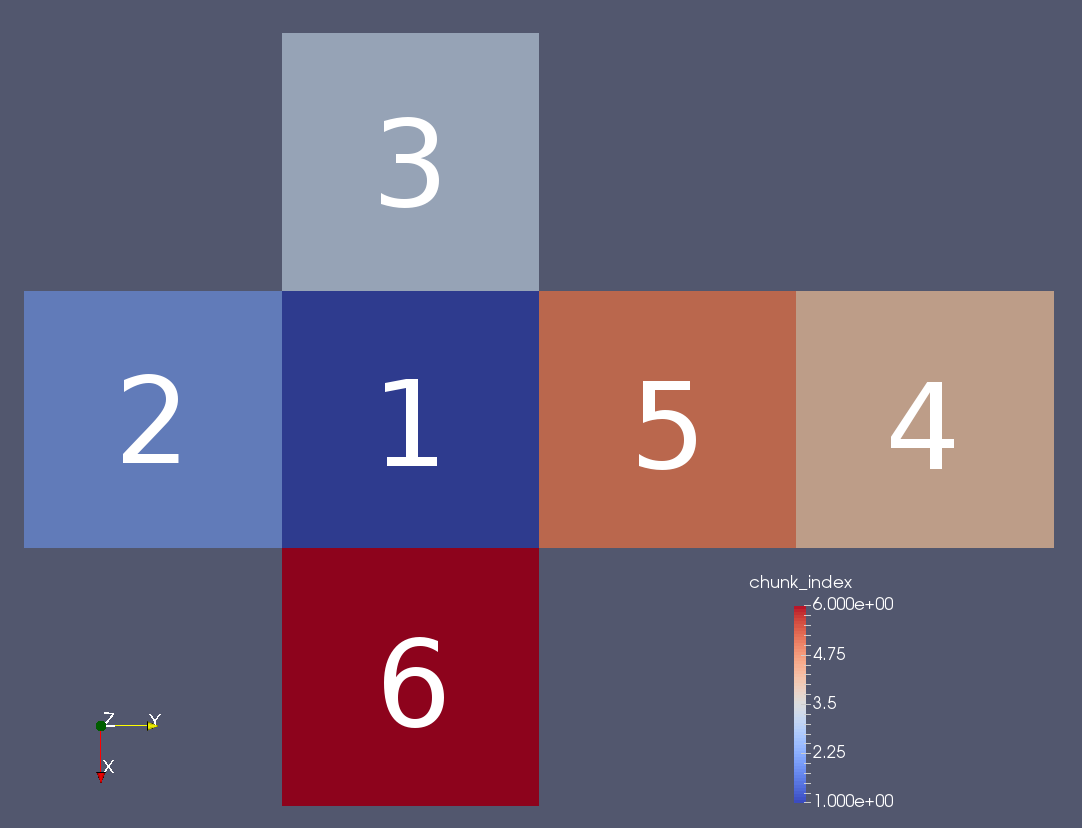
\includegraphics[width=0.65\textwidth]{images/chunksInversionGrid_6-chunks_ichunk_LOCAL_FLAT_numbers.png}
  \caption{distribution of chunks of the chunksInversionGrid in \lcode{LOCAL_FLAT} projection}
  \label{ssec-invgrid:chunks-cell-ref,fig:ichunk}
\end{figure}

In order to make \ASKI{} support a new method of base cell refinement for inversion grids of type 
\lcode{chunksInversionGrid}, module \lcode{chunksInversionGrid} must be extended, as indicated by comments
\begin{verbatim}
!##################################
! ADD YOUR REFINEMENT METHOD HERE
!##################################
\end{verbatim}
in file \lcode{chunksInversionGrid.f90}. In particular,
\begin{itemize}
\item In routine \lcode{readCheckParFileChunksInversionGrid}, the new value of keyword 
  \lcode{CHUNKS_INVGRID_CREF_METHOD} (name of refinement method) must pass all checks and (if required) any 
  expected values must be read from keyword \lcode{CHUNKS_INVGRID_CREF_PARAMETERS}.
  Alternatively, you may need to introduce another keyword to read in some filenames
  or introduce some naming convention for files containing additional information.
\item Routine \lcode{doCellRefinementChunksInversionGrid} must execute one or more new subroutines (to be 
  implemented specifically for the new refinement method) which do the actual refinement, as described in
  the commented toy subroutine \\\lcode{requiredSubroutinesForNewRefinementMethod}.
\end{itemize}
 

%-------------------------------
% SECTION todo / new ideas / pending things to implmement
%#############################################################
\section{Things ``to do'' for the \ASKI{} developers} \label{sec:todo}
%#############################################################
Please make sure to remove those aspects from this section of the \ASKI{} developers manual which you have fixed.

%-------------------------------------
\subsection{Todos that are straightforward to realize} \label{ssec-todo:todo-simple}
%-------------------------------------

\subsubsection{use function \lcodetitle{nextPathDataModelSpaceInfo} everywhere}
%
Originally, loops over event-station paths were done manually (by first getting the paths by 
\lcode{getPathsDataModelSpaceInfo} and then looping over them). Some of these implementations might
be more clear if a construct like\\
\lcode{do while( nextPathDataModelSpaceInfo(...) )}\\
was used, \emph{directly} accessing information on components and frequencies via function 
\lcode{nextPathDataModelSpaceInfo} (instead of using \lcode{getIndxDataSamples} inside the manual loop 
over the paths).

Especially in the module \lcode{dataModelSpaceInfo} itself, the old approach (looping over paths manually) is
done thoroughly, as well as in \lcode{investigateDataResiduals} (sensible also for 
\lcode{computeDataFromKernelSystem}?!)

\subsubsection{finish implementing module \lcodetitle{parameterCorrelation}}
%
So far, there is only a quick hack done for constructing objects (for reasons of testing):
In the parameter correlation file as given by the main parameter file, assume only ONE line, 
containing for parameter vs the parameters of  rho , vp (in that order, space separated).
Please refer to comments in code file \lcode{parameterCorrelation.f90} containing \lcode{FS FS}
(always referring to author Florian Schumacher).

%-------------------------------------
\subsection{Todos that might require some more work} \label{ssec-todo:todo-complex}
%-------------------------------------
\subsubsection{completion of module \lcodetitle{ecartInversionGrid}}
The module \lcode{ecartInversionGrid} is exensively (!) documented in the code file \lcode{ecartInversionGrid.f90},
mostly \emph{without} doxygen syntax (so you can only access the documentation by reading the code file's commentary
sections).

The following subroutines/functionality must still be implemented for \emph{hexahedral} (i.e.\ \lcode{hex8}) cells:
\begin{enumerate}
\item \lcode{locateWpInsideHex8CellEcartInversionGrid}
\item \lcode{transformToStandardHexEcartInversionGrid}
\item \lcode{getVolumeHex8EcartInversionGrid}
\item \lcode{createFaceNeighboursEcartInversionGrid}: only face neighbours are searched for among \lcode{tet4}
  cells, \emph{which still is unstable, see below}. Still to do: include \lcode{hex8} cells in the
  search, i.e.\ search for neighbours among \lcode{hex8} cells \emph{and} between \lcode{hex8} and \lcode{tet4} cells.\\
  \emph{Alternatively}, a neighbour search (i.e.\ creation of the neighbours file) could be done outside this module by 
  arbitrary software, e.g.\ already at the stage of exporting the grid from Trelis (if possible?!) by script 
  \lcode{cubit2ASKIecartInversionGrid.py}.
\end{enumerate}

Also, the neighbour search among the \lcode{tet4} cells in subroutine \lcode{createFaceNeighboursEcartInversionGrid} 
(following the approach of testing signed areas of triangles which are spanned by one point of the first tri face 
and an edge of the other tri face, as described in section 4 of paper \cite{devillers:inria-00072100}) 
turned out to be still unstable and must be fixed: please compare example files and \lcode{README} in\\
\lcode{doc/ASKI_developers_manual/TODO_ecartInversionGrid_cell_neighbours/}\\
(the inversion grid given there is also given as an example in the user manual and in
\lcode{doc/example_ecartInversionGrid/}, as of August 2016).
For some \lcode{tet4} cells not all neighbours are found correctly, for some cells not even one of the neighbours
is found. The reason for that should be due to the numerical implementation of the search algorithm (possibly 
problems comparing floating point numbers).

\subsubsection{improvement of the \ASKI{} user manual, section entitled ``What is \ASKI{}?''}
We might include some pictures there: a set of points inside the volumes 
of the inversion grid, a sensitivity kernel for one specific datum (real part of some frequency 
sample of a seismogram (src,rec,comp)) explaining that positive high values at one scatterer mean 
that this very datum increases (significantly) if the current model parameter is increased at this scatterer, etc.

%-------------------------------------
\subsection{Ideas for new \ASKI{} functionality} \label{ssec-todo:new}
%-------------------------------------
\subsubsection{file-interface to module \lcodetitle{dataModelSpaceInfo}}
The parsing of dataModelSpaceInfo files in module \lcode{dataModelSpaceInfo} (routine 
\lcode{createFromFileDataModelSpaceInfo}) is very inconvenient (as it is implemented in Fortran).
Alternatively (as an \emph{additional} feature!), module \lcode{dataModelSpaceInfo} can support to read in
a text file that contains listed information of all data samples and/or model values (maybe two separate files
for data samples and model values?!), i.e.\ basically arrays \lcode{evid}, \lcode{staname}, \lcode{comp}, 
\lcode{ifreq}, \lcode{imre}, \lcode{wdata}, \lcode{normalization_mdata}, \lcode{normalization_sdata}, 
\lcode{normalization_kernel}, as columns (for model values file: this means arrays \lcode{param}, \lcode{cell}, 
respectively). Also memorize values like \lcode{ndata}, \lcode{nmval}, \lcode{parametrization} in these files.
\emph{Additionally} on could remember in these files information like paths, number of paths,
which receiver components, frequencies are contained in which paths, 
all different comp, all different ifreq, etc.
The best thing would be to memorize all (or a lot of) information required by 
the programs, e.g.\ all data indices per path, etc. This could allow for quicker access in the application 
of the programs (although everything is working now).

\subsubsection{forward-method interface modules for synthetic data}
It would be much better to have a set of interface modules for synthetic data (just as
for wavefield points, kernel reference model, kernel displacement, kernel Green tensor), because the forward code
requires knowledge about the \ASKI{}-internal file format of synthetic data. These interface modules of synthetic
data could use the \lcode{discreteFourierTransform} module (if required) and know the location, name and format 
of any synthetic data files written by the forward code.

\subsubsection{support integer list of formats like ``3-5,9,13,19-21''}
For some input on the command line (the \ASKI{} Fortran executables usually use the module \lcode{argumentParser}), 
explicit vectors of integer values are required (e.g. \lcode{-subs} of executable \lcode{chunksInvgrid2vtk}). At 
the moment, all indices have to be given on the command line explicitely (space-separated). Usually one has to apply 
quotes like \\
\lcode{-subs "3 4 5 9 13 19 20 21"}\\
This can get very long and lengthy and unconvenient for a user that does not want to use option \lcode{-all_subs}.

Such integer vectors are also used in another respect in \ASKI{}, namely for defining frequency indices in 
parameter files (main parameter file and iteration-step-specific parameter file). If an input line there
becomes too long (because of so many space-separated items in the line), it might even not be possible to read 
this line properly by module \lcode{inputParameter}, since it uses a maximum character length for value strings
of 500.

This functionality could be realized by implementing a new module (called something like \lcode{integerRanges})
which knows how to transform strings of form ``3-5,9,13,19-21'' to integer arrays \lcode{3 4 5 9 13 19 20 21}.
This module could even support different kinds of string formatting which it automatically detects (if it does
not detect a known format, it returns an error).
It is thinkable to also support formats like \lcode{all-except:3-5,9,13,19-21}, but in this case it must be clear
to module \lcode{integerRanges} what ``all'' means, i.e.\ to which entirety the numbers refer.

\subsubsection{other methods of smoothing kernel inverted models}
In module \lcode{linearModelRegularization} the only supported smoothing method at the moment is implemented in subroutine 
\lcode{addNeighbourAverageSmoothingLinearModelRegularization} and builds averages over direct face neighbours
(possibly accounting for different boundary conditions on boundaries where there are no neighbours or boundaries
that should not be smoothed over (last aspect not yet implemented but possible after somehow defining internal 
boundaries)).

An alternative method that \emph{does not require neighbour information} and is more physically motivated is 
suggested in the following:
\begin{itemize}
\item Given a fixed radius $r$, detect for each inversion grid cell $c$ all other cells $c_n$ for which the
  distance between the center points of $c$ and $c_n$ is $\le r$ (regard those cells as ``neighbours'' in this 
  sense, i.e. ``central-radius-neighbours'', although they do not need to be \emph{face} neighbours in the 
  above sence). This detection of ``closeby'' cells
  should be implemented in module \lcode{inversionGrid} and its containing submodules as an alternative ``neighbour search''
  called something like \lcode{getIndicesCentralRadiusNeighboursInversionGrid}
\item Then build smoothing conditions as averages on all central-radius-neighbours. Optionally, the weight $w_n$
  of neighbour $c_n$ in the linear combination of this average may depend on the distance between center points of
  $c$ and $c_n$ (as a result: cell further away have a smaller influence on the smoothed value).
\item As an alternative to searching for central-radius-neighbours by a fixed radius $r$ (constant $r$ throughout 
  the inversion grid, regardless of the spatial extent of inversion grid cell $c$ which constitutes the local 
  spatial resolution of the inversion grid), the search may be performed by a dynamic radius $r_c$ which 
  depends on the particular inversion grid cell $c$ for which neighbours should be found. $r_c$ may e.g.\ be computed
  by multiplying the radius of cell $c$ by a fixed given factor $f>1$ (constand $f$ throughout the inversion grid).
  Thereby, the influence of the smoothing operation would correspond to the local spatial resolution of the 
  inversion grid (in regions of finer spatial resolution, the smoothing would have a smaller range of influence, 
  in regions with coarser spatial resolution, the model values on the inversion grid cells would depend on values
  at larger distances). This variety of the central-radius neighbours search comes closes to the search of face
  neighbours.
\end{itemize}



%
%-------------------------------
% BIBLIOGRAPHY
\bibliographystyle{alpha}
\bibliography{bibliography}
\phantomsection  % so hyperref creates bookmarks
\addcontentsline{toc}{section}{References}
%
%-------------------------------
% SECTION History (of the document versions, as required by the GNU Free Documentation License)
\newpage
\section*{History}
\phantomsection  % so hyperref creates bookmarks
\addcontentsline{toc}{section}{History}
% -*-LaTex-*-

%-----------------------------------------------------------------------------
%   Copyright 2016 Florian Schumacher
%
%   This file is part of the ASKI manual as a LaTeX document with main file
%   manual.tex
%
%   Permission is granted to copy, distribute and/or modify this document
%   under the terms of the GNU Free Documentation License, Version 1.3
%   or any later version published by the Free Software Foundation;
%   with no Invariant Sections, no Front-Cover Texts, and no Back-Cover Texts.
%   A copy of the license is included in the section entitled ``GNU
%   Free Documentation License''. 
%-----------------------------------------------------------------------------
%
This is a section on the history of this document, i.e.\ its previously published versions, as referred to by
the GNU Free Documentation License (version 1.3).

%-------------------------------
% Manual for ASKI version 1.2, August 2016
\subsection*{ASKI User Manual, ASKI version 1.2, August 2016}

Recognizable snippet from the title page (scaled):

\begin{minipage}{0.45\textwidth}
  \begin{flushright} \tt
      {\LARGE User Manual} \\[1em]
      {\large ASKI} {\rm --} version 1.2 \\[1em]
      Aug 2016 \\
      Florian Schumacher \\ 
      {\footnotesize Ruhr-Universit\"at Bochum, Germany}
  \end{flushright}
\end{minipage}
\vspace*{1ex}

{\bf Title: } ASKI User Manual, ASKI version 1.2, August 2016\\
{\bf Year: } 2016\\
{\bf Authors: } Florian Schumacher (Ruhr-Universit\"at Bochum, Germany)

This version of this document is provided for download (as of August 2016) at\\
\url{https://github.com/seismology-RUB/ASKI/releases/tag/v1.2}\\
Direct link (as of August 2016):\\
\url{https://github.com/seismology-RUB/ASKI/releases/download/v1.2/ASKI_manual_1-2_aug-2016.pdf}


%-------------------------------
% Manual for ASKI version 1.1, March 2016
\subsection*{ASKI user manual, ASKI version 1.1, March 2016}

Recognizable snippet from the title page (scaled):

\begin{minipage}{0.45\textwidth}
  \begin{flushright} \tt
      {\LARGE User Manual} \\[1em]
      {\large ASKI} {\rm --} version 1.1 \\[1em]
      Mar 2016 \\
      Florian Schumacher \\ 
      {\footnotesize Ruhr-Universit\"at Bochum, Germany}
  \end{flushright}
\end{minipage}
\vspace*{1ex}

{\bf Title: } ASKI User Manual, ASKI version 1.1, March 2016\\
{\bf Year: } 2016\\
{\bf Authors: } Florian Schumacher (Ruhr-Universit\"at Bochum, Germany)

This version of this document is provided for download (as of August 2016) at\\
\url{https://github.com/seismology-RUB/ASKI/releases/tag/v1.1}\\
Direct link (as of August 2016):\\
\url{https://github.com/seismology-RUB/ASKI/releases/download/v1.1/ASKI_manual_1-1_mar-2016.pdf}


%-------------------------------
% Manual for ASKI version 1.0, December 2015
\subsection*{ASKI user manual, ASKI version 1.0, December 2015}

Recognizable snippet from the title page (scaled):

\begin{minipage}{0.45\textwidth}
  \begin{flushright} \tt
      {\LARGE User Manual} \\[1em]
      {\large ASKI} {\rm --} version 1.0 \\[1em]
      Dec 2015 \\
      Florian Schumacher \\ 
      {\footnotesize Ruhr-Universit\"at Bochum, Germany}
  \end{flushright}
\end{minipage}
\vspace*{1ex}

{\bf Title: } ASKI User Manual, ASKI version 1.0, December 2015\\
{\bf Year: } 2015\\
{\bf Authors: } Florian Schumacher (Ruhr-Universit\"at Bochum, Germany)

This version of this document is provided for download (as of August 2016) at\\
\url{https://github.com/seismology-RUB/ASKI/releases/tag/v1.0}\\
Direct link (as of August 2016):\\
\url{https://github.com/seismology-RUB/ASKI/releases/download/v1.0/ASKI_manual_1-0_dec-2015.pdf}


%-------------------------------
% Manual for ASKI version 0.3, 2013
\subsection*{ASKI user manual, ASKI version 0.3, 2013}

Recognizable snippet from the title page (scaled):

\begin{minipage}{0.45\textwidth}
  \begin{flushright} \tt
      {\LARGE User Manual} \\[1em]
      {\large ASKI} {\rm --} version 0.3 \\[1em]
      2013 \\
      Florian Schumacher \\ 
      {\footnotesize Ruhr-Universit\"at Bochum, Germany}
  \end{flushright}
\end{minipage}
\vspace*{1ex}

{\bf Title: } ASKI User Manual, ASKI version 0.3, 2013\\
{\bf Year: } 2013\\
{\bf Authors: } Florian Schumacher (Ruhr-Universit\"at Bochum, Germany)

This version of this document is provided for download (as of August 2016) at\\
\url{https://github.com/seismology-RUB/ASKI/releases/tag/v0.3}\\
being contained in the provided \lcode{.zip} code archive as file \\
\lcode{ASKI-0.3/doc/ASKI_manual.pdf}\\
Direct link (as of August 2016):\\
\url{https://github.com/seismology-RUB/ASKI/archive/v0.3.zip}


%
%-------------------------------
% SECTION GNU Free Documentation License
\newpage
%-----------------------------------------------------------------------------
%   Copyright 2013 Florian Schumacher
%
%   This file is part of the ASKI manual as a LaTeX document with main file
%   manual.tex
%
%   Permission is granted to copy, distribute and/or modify this document
%   under the terms of the GNU Free Documentation License, Version 1.3
%   or any later version published by the Free Software Foundation;
%   with no Invariant Sections, no Front-Cover Texts, and no Back-Cover Texts.
%   A copy of the license is included in the section entitled ``GNU
%   Free Documentation License''. 
%-----------------------------------------------------------------------------
%   The following content of the file is a verbatim copy of file 
%   http://www.gnu.org/licenses/fdl-1.3.tex which has been slightly modified in 
%   terms of hyperref bookmarks and uncommenting the document preamble in order 
%   to fit the needs embedding it in the ASKI manual as a LaTeX document with 
%   main file manual.tex
%   2013, Florian Schumacher
%-----------------------------------------------------------------------------
%
%% This is set up to run with pdflatex.
%%---------The file header---------------------------------------------
%\documentclass[a4paper,12pt]{book}
%
%\usepackage[english]{babel} %language selection
%\selectlanguage{english}
%
%\pagenumbering{arabic}
%
%\usepackage{hyperref}
%\hypersetup{colorlinks, 
%           citecolor=black,
%           filecolor=black,
%           linkcolor=black,
%           urlcolor=black,
%           bookmarksopen=true,
%           pdftex}
%
%\hfuzz = .6pt % avoid black boxes
%           
%\begin{document}
%%---------------------------------------------------------------------
\chapter*{\rlap{GNU Free Documentation License}}
\phantomsection  % so hyperref creates bookmarks
\addcontentsline{toc}{chapter}{GNU Free Documentation License}
\label{label_fdl}

 \begin{center}

       Version 1.3, 3 November 2008


 Copyright \copyright{} 2000, 2001, 2002, 2007, 2008  Free Software Foundation, Inc.
 
 \bigskip
 
     \texttt{<http://fsf.org/>}
  
 \bigskip
 
 Everyone is permitted to copy and distribute verbatim copies
 of this license document, but changing it is not allowed.
\end{center}


\begin{center}
{\bf\large Preamble}
\end{center}

The purpose of this License is to make a manual, textbook, or other
functional and useful document ``free'' in the sense of freedom: to
assure everyone the effective freedom to copy and redistribute it,
with or without modifying it, either commercially or noncommercially.
Secondarily, this License preserves for the author and publisher a way
to get credit for their work, while not being considered responsible
for modifications made by others.

This License is a kind of ``copyleft'', which means that derivative
works of the document must themselves be free in the same sense.  It
complements the GNU General Public License, which is a copyleft
license designed for free software.

We have designed this License in order to use it for manuals for free
software, because free software needs free documentation: a free
program should come with manuals providing the same freedoms that the
software does.  But this License is not limited to software manuals;
it can be used for any textual work, regardless of subject matter or
whether it is published as a printed book.  We recommend this License
principally for works whose purpose is instruction or reference.


\begin{center}
{\Large\bf 1. APPLICABILITY AND DEFINITIONS\par}
\phantomsection
%\addcontentsline{toc}{section}{1. APPLICABILITY AND DEFINITIONS}
\end{center}

This License applies to any manual or other work, in any medium, that
contains a notice placed by the copyright holder saying it can be
distributed under the terms of this License.  Such a notice grants a
world-wide, royalty-free license, unlimited in duration, to use that
work under the conditions stated herein.  The ``\textbf{Document}'', below,
refers to any such manual or work.  Any member of the public is a
licensee, and is addressed as ``\textbf{you}''.  You accept the license if you
copy, modify or distribute the work in a way requiring permission
under copyright law.

A ``\textbf{Modified Version}'' of the Document means any work containing the
Document or a portion of it, either copied verbatim, or with
modifications and/or translated into another language.

A ``\textbf{Secondary Section}'' is a named appendix or a front-matter section of
the Document that deals exclusively with the relationship of the
publishers or authors of the Document to the Document's overall subject
(or to related matters) and contains nothing that could fall directly
within that overall subject.  (Thus, if the Document is in part a
textbook of mathematics, a Secondary Section may not explain any
mathematics.)  The relationship could be a matter of historical
connection with the subject or with related matters, or of legal,
commercial, philosophical, ethical or political position regarding
them.

The ``\textbf{Invariant Sections}'' are certain Secondary Sections whose titles
are designated, as being those of Invariant Sections, in the notice
that says that the Document is released under this License.  If a
section does not fit the above definition of Secondary then it is not
allowed to be designated as Invariant.  The Document may contain zero
Invariant Sections.  If the Document does not identify any Invariant
Sections then there are none.

The ``\textbf{Cover Texts}'' are certain short passages of text that are listed,
as Front-Cover Texts or Back-Cover Texts, in the notice that says that
the Document is released under this License.  A Front-Cover Text may
be at most 5 words, and a Back-Cover Text may be at most 25 words.

A ``\textbf{Transparent}'' copy of the Document means a machine-readable copy,
represented in a format whose specification is available to the
general public, that is suitable for revising the document
straightforwardly with generic text editors or (for images composed of
pixels) generic paint programs or (for drawings) some widely available
drawing editor, and that is suitable for input to text formatters or
for automatic translation to a variety of formats suitable for input
to text formatters.  A copy made in an otherwise Transparent file
format whose markup, or absence of markup, has been arranged to thwart
or discourage subsequent modification by readers is not Transparent.
An image format is not Transparent if used for any substantial amount
of text.  A copy that is not ``Transparent'' is called ``\textbf{Opaque}''.

Examples of suitable formats for Transparent copies include plain
ASCII without markup, Texinfo input format, LaTeX input format, SGML
or XML using a publicly available DTD, and standard-conforming simple
HTML, PostScript or PDF designed for human modification.  Examples of
transparent image formats include PNG, XCF and JPG.  Opaque formats
include proprietary formats that can be read and edited only by
proprietary word processors, SGML or XML for which the DTD and/or
processing tools are not generally available, and the
machine-generated HTML, PostScript or PDF produced by some word
processors for output purposes only.

The ``\textbf{Title Page}'' means, for a printed book, the title page itself,
plus such following pages as are needed to hold, legibly, the material
this License requires to appear in the title page.  For works in
formats which do not have any title page as such, ``Title Page'' means
the text near the most prominent appearance of the work's title,
preceding the beginning of the body of the text.

The ``\textbf{publisher}'' means any person or entity that distributes
copies of the Document to the public.

A section ``\textbf{Entitled XYZ}'' means a named subunit of the Document whose
title either is precisely XYZ or contains XYZ in parentheses following
text that translates XYZ in another language.  (Here XYZ stands for a
specific section name mentioned below, such as ``\textbf{Acknowledgements}'',
``\textbf{Dedications}'', ``\textbf{Endorsements}'', or ``\textbf{History}''.)  
To ``\textbf{Preserve the Title}''
of such a section when you modify the Document means that it remains a
section ``Entitled XYZ'' according to this definition.

The Document may include Warranty Disclaimers next to the notice which
states that this License applies to the Document.  These Warranty
Disclaimers are considered to be included by reference in this
License, but only as regards disclaiming warranties: any other
implication that these Warranty Disclaimers may have is void and has
no effect on the meaning of this License.


\begin{center}
{\Large\bf 2. VERBATIM COPYING\par}
\phantomsection
%\addcontentsline{toc}{section}{2. VERBATIM COPYING}
\end{center}

You may copy and distribute the Document in any medium, either
commercially or noncommercially, provided that this License, the
copyright notices, and the license notice saying this License applies
to the Document are reproduced in all copies, and that you add no other
conditions whatsoever to those of this License.  You may not use
technical measures to obstruct or control the reading or further
copying of the copies you make or distribute.  However, you may accept
compensation in exchange for copies.  If you distribute a large enough
number of copies you must also follow the conditions in section~3.

You may also lend copies, under the same conditions stated above, and
you may publicly display copies.


\begin{center}
{\Large\bf 3. COPYING IN QUANTITY\par}
\phantomsection
%\addcontentsline{toc}{section}{3. COPYING IN QUANTITY}
\end{center}


If you publish printed copies (or copies in media that commonly have
printed covers) of the Document, numbering more than 100, and the
Document's license notice requires Cover Texts, you must enclose the
copies in covers that carry, clearly and legibly, all these Cover
Texts: Front-Cover Texts on the front cover, and Back-Cover Texts on
the back cover.  Both covers must also clearly and legibly identify
you as the publisher of these copies.  The front cover must present
the full title with all words of the title equally prominent and
visible.  You may add other material on the covers in addition.
Copying with changes limited to the covers, as long as they preserve
the title of the Document and satisfy these conditions, can be treated
as verbatim copying in other respects.

If the required texts for either cover are too voluminous to fit
legibly, you should put the first ones listed (as many as fit
reasonably) on the actual cover, and continue the rest onto adjacent
pages.

If you publish or distribute Opaque copies of the Document numbering
more than 100, you must either include a machine-readable Transparent
copy along with each Opaque copy, or state in or with each Opaque copy
a computer-network location from which the general network-using
public has access to download using public-standard network protocols
a complete Transparent copy of the Document, free of added material.
If you use the latter option, you must take reasonably prudent steps,
when you begin distribution of Opaque copies in quantity, to ensure
that this Transparent copy will remain thus accessible at the stated
location until at least one year after the last time you distribute an
Opaque copy (directly or through your agents or retailers) of that
edition to the public.

It is requested, but not required, that you contact the authors of the
Document well before redistributing any large number of copies, to give
them a chance to provide you with an updated version of the Document.


\begin{center}
{\Large\bf 4. MODIFICATIONS\par}
\phantomsection
%\addcontentsline{toc}{section}{4. MODIFICATIONS}
\end{center}

You may copy and distribute a Modified Version of the Document under
the conditions of sections 2 and 3 above, provided that you release
the Modified Version under precisely this License, with the Modified
Version filling the role of the Document, thus licensing distribution
and modification of the Modified Version to whoever possesses a copy
of it.  In addition, you must do these things in the Modified Version:

\begin{itemize}
\item[A.] 
   Use in the Title Page (and on the covers, if any) a title distinct
   from that of the Document, and from those of previous versions
   (which should, if there were any, be listed in the History section
   of the Document).  You may use the same title as a previous version
   if the original publisher of that version gives permission.
   
\item[B.]
   List on the Title Page, as authors, one or more persons or entities
   responsible for authorship of the modifications in the Modified
   Version, together with at least five of the principal authors of the
   Document (all of its principal authors, if it has fewer than five),
   unless they release you from this requirement.
   
\item[C.]
   State on the Title page the name of the publisher of the
   Modified Version, as the publisher.
   
\item[D.]
   Preserve all the copyright notices of the Document.
   
\item[E.]
   Add an appropriate copyright notice for your modifications
   adjacent to the other copyright notices.
   
\item[F.]
   Include, immediately after the copyright notices, a license notice
   giving the public permission to use the Modified Version under the
   terms of this License, in the form shown in the Addendum below.
   
\item[G.]
   Preserve in that license notice the full lists of Invariant Sections
   and required Cover Texts given in the Document's license notice.
   
\item[H.]
   Include an unaltered copy of this License.
   
\item[I.]
   Preserve the section Entitled ``History'', Preserve its Title, and add
   to it an item stating at least the title, year, new authors, and
   publisher of the Modified Version as given on the Title Page.  If
   there is no section Entitled ``History'' in the Document, create one
   stating the title, year, authors, and publisher of the Document as
   given on its Title Page, then add an item describing the Modified
   Version as stated in the previous sentence.
   
\item[J.]
   Preserve the network location, if any, given in the Document for
   public access to a Transparent copy of the Document, and likewise
   the network locations given in the Document for previous versions
   it was based on.  These may be placed in the ``History'' section.
   You may omit a network location for a work that was published at
   least four years before the Document itself, or if the original
   publisher of the version it refers to gives permission.
   
\item[K.]
   For any section Entitled ``Acknowledgements'' or ``Dedications'',
   Preserve the Title of the section, and preserve in the section all
   the substance and tone of each of the contributor acknowledgements
   and/or dedications given therein.
   
\item[L.]
   Preserve all the Invariant Sections of the Document,
   unaltered in their text and in their titles.  Section numbers
   or the equivalent are not considered part of the section titles.
   
\item[M.]
   Delete any section Entitled ``Endorsements''.  Such a section
   may not be included in the Modified Version.
   
\item[N.]
   Do not retitle any existing section to be Entitled ``Endorsements''
   or to conflict in title with any Invariant Section.
   
\item[O.]
   Preserve any Warranty Disclaimers.
\end{itemize}

If the Modified Version includes new front-matter sections or
appendices that qualify as Secondary Sections and contain no material
copied from the Document, you may at your option designate some or all
of these sections as invariant.  To do this, add their titles to the
list of Invariant Sections in the Modified Version's license notice.
These titles must be distinct from any other section titles.

You may add a section Entitled ``Endorsements'', provided it contains
nothing but endorsements of your Modified Version by various
parties---for example, statements of peer review or that the text has
been approved by an organization as the authoritative definition of a
standard.

You may add a passage of up to five words as a Front-Cover Text, and a
passage of up to 25 words as a Back-Cover Text, to the end of the list
of Cover Texts in the Modified Version.  Only one passage of
Front-Cover Text and one of Back-Cover Text may be added by (or
through arrangements made by) any one entity.  If the Document already
includes a cover text for the same cover, previously added by you or
by arrangement made by the same entity you are acting on behalf of,
you may not add another; but you may replace the old one, on explicit
permission from the previous publisher that added the old one.

The author(s) and publisher(s) of the Document do not by this License
give permission to use their names for publicity for or to assert or
imply endorsement of any Modified Version.


\begin{center}
{\Large\bf 5. COMBINING DOCUMENTS\par}
\phantomsection
%\addcontentsline{toc}{section}{5. COMBINING DOCUMENTS}
\end{center}


You may combine the Document with other documents released under this
License, under the terms defined in section~4 above for modified
versions, provided that you include in the combination all of the
Invariant Sections of all of the original documents, unmodified, and
list them all as Invariant Sections of your combined work in its
license notice, and that you preserve all their Warranty Disclaimers.

The combined work need only contain one copy of this License, and
multiple identical Invariant Sections may be replaced with a single
copy.  If there are multiple Invariant Sections with the same name but
different contents, make the title of each such section unique by
adding at the end of it, in parentheses, the name of the original
author or publisher of that section if known, or else a unique number.
Make the same adjustment to the section titles in the list of
Invariant Sections in the license notice of the combined work.

In the combination, you must combine any sections Entitled ``History''
in the various original documents, forming one section Entitled
``History''; likewise combine any sections Entitled ``Acknowledgements'',
and any sections Entitled ``Dedications''.  You must delete all sections
Entitled ``Endorsements''.

\begin{center}
{\Large\bf 6. COLLECTIONS OF DOCUMENTS\par}
\phantomsection
%\addcontentsline{toc}{section}{6. COLLECTIONS OF DOCUMENTS}
\end{center}

You may make a collection consisting of the Document and other documents
released under this License, and replace the individual copies of this
License in the various documents with a single copy that is included in
the collection, provided that you follow the rules of this License for
verbatim copying of each of the documents in all other respects.

You may extract a single document from such a collection, and distribute
it individually under this License, provided you insert a copy of this
License into the extracted document, and follow this License in all
other respects regarding verbatim copying of that document.


\begin{center}
{\Large\bf 7. AGGREGATION WITH INDEPENDENT WORKS\par}
\phantomsection
%\addcontentsline{toc}{section}{7. AGGREGATION WITH INDEPENDENT WORKS}
\end{center}


A compilation of the Document or its derivatives with other separate
and independent documents or works, in or on a volume of a storage or
distribution medium, is called an ``aggregate'' if the copyright
resulting from the compilation is not used to limit the legal rights
of the compilation's users beyond what the individual works permit.
When the Document is included in an aggregate, this License does not
apply to the other works in the aggregate which are not themselves
derivative works of the Document.

If the Cover Text requirement of section~3 is applicable to these
copies of the Document, then if the Document is less than one half of
the entire aggregate, the Document's Cover Texts may be placed on
covers that bracket the Document within the aggregate, or the
electronic equivalent of covers if the Document is in electronic form.
Otherwise they must appear on printed covers that bracket the whole
aggregate.


\begin{center}
{\Large\bf 8. TRANSLATION\par}
\phantomsection
%\addcontentsline{toc}{section}{8. TRANSLATION}
\end{center}


Translation is considered a kind of modification, so you may
distribute translations of the Document under the terms of section~4.
Replacing Invariant Sections with translations requires special
permission from their copyright holders, but you may include
translations of some or all Invariant Sections in addition to the
original versions of these Invariant Sections.  You may include a
translation of this License, and all the license notices in the
Document, and any Warranty Disclaimers, provided that you also include
the original English version of this License and the original versions
of those notices and disclaimers.  In case of a disagreement between
the translation and the original version of this License or a notice
or disclaimer, the original version will prevail.

If a section in the Document is Entitled ``Acknowledgements'',
``Dedications'', or ``History'', the requirement (section~4) to Preserve
its Title (section~1) will typically require changing the actual
title.


\begin{center}
{\Large\bf 9. TERMINATION\par}
\phantomsection
%\addcontentsline{toc}{section}{9. TERMINATION}
\end{center}


You may not copy, modify, sublicense, or distribute the Document
except as expressly provided under this License.  Any attempt
otherwise to copy, modify, sublicense, or distribute it is void, and
will automatically terminate your rights under this License.

However, if you cease all violation of this License, then your license
from a particular copyright holder is reinstated (a) provisionally,
unless and until the copyright holder explicitly and finally
terminates your license, and (b) permanently, if the copyright holder
fails to notify you of the violation by some reasonable means prior to
60 days after the cessation.

Moreover, your license from a particular copyright holder is
reinstated permanently if the copyright holder notifies you of the
violation by some reasonable means, this is the first time you have
received notice of violation of this License (for any work) from that
copyright holder, and you cure the violation prior to 30 days after
your receipt of the notice.

Termination of your rights under this section does not terminate the
licenses of parties who have received copies or rights from you under
this License.  If your rights have been terminated and not permanently
reinstated, receipt of a copy of some or all of the same material does
not give you any rights to use it.


\begin{center}
{\Large\bf 10. FUTURE REVISIONS OF THIS LICENSE\par}
\phantomsection
%\addcontentsline{toc}{section}{10. FUTURE REVISIONS OF THIS LICENSE}
\end{center}


The Free Software Foundation may publish new, revised versions
of the GNU Free Documentation License from time to time.  Such new
versions will be similar in spirit to the present version, but may
differ in detail to address new problems or concerns.  See
\texttt{http://www.gnu.org/copyleft/}.

Each version of the License is given a distinguishing version number.
If the Document specifies that a particular numbered version of this
License ``or any later version'' applies to it, you have the option of
following the terms and conditions either of that specified version or
of any later version that has been published (not as a draft) by the
Free Software Foundation.  If the Document does not specify a version
number of this License, you may choose any version ever published (not
as a draft) by the Free Software Foundation.  If the Document
specifies that a proxy can decide which future versions of this
License can be used, that proxy's public statement of acceptance of a
version permanently authorizes you to choose that version for the
Document.


\begin{center}
{\Large\bf 11. RELICENSING\par}
\phantomsection
%\addcontentsline{toc}{section}{11. RELICENSING}
\end{center}


``Massive Multiauthor Collaboration Site'' (or ``MMC Site'') means any
World Wide Web server that publishes copyrightable works and also
provides prominent facilities for anybody to edit those works.  A
public wiki that anybody can edit is an example of such a server.  A
``Massive Multiauthor Collaboration'' (or ``MMC'') contained in the
site means any set of copyrightable works thus published on the MMC
site.

``CC-BY-SA'' means the Creative Commons Attribution-Share Alike 3.0
license published by Creative Commons Corporation, a not-for-profit
corporation with a principal place of business in San Francisco,
California, as well as future copyleft versions of that license
published by that same organization.

``Incorporate'' means to publish or republish a Document, in whole or
in part, as part of another Document.

An MMC is ``eligible for relicensing'' if it is licensed under this
License, and if all works that were first published under this License
somewhere other than this MMC, and subsequently incorporated in whole
or in part into the MMC, (1) had no cover texts or invariant sections,
and (2) were thus incorporated prior to November 1, 2008.

The operator of an MMC Site may republish an MMC contained in the site
under CC-BY-SA on the same site at any time before August 1, 2009,
provided the MMC is eligible for relicensing.


\begin{center}
{\Large\bf ADDENDUM: How to use this License for your documents\par}
\phantomsection
%\addcontentsline{toc}{section}{ADDENDUM: How to use this License for your documents}
\end{center}

To use this License in a document you have written, include a copy of
the License in the document and put the following copyright and
license notices just after the title page:

\bigskip
\begin{quote}
    Copyright \copyright{}  YEAR  YOUR NAME.
    Permission is granted to copy, distribute and/or modify this document
    under the terms of the GNU Free Documentation License, Version 1.3
    or any later version published by the Free Software Foundation;
    with no Invariant Sections, no Front-Cover Texts, and no Back-Cover Texts.
    A copy of the license is included in the section entitled ``GNU
    Free Documentation License''.
\end{quote}
\bigskip
    
If you have Invariant Sections, Front-Cover Texts and Back-Cover Texts,
replace the ``with \dots\ Texts.''\ line with this:

\bigskip
\begin{quote}
    with the Invariant Sections being LIST THEIR TITLES, with the
    Front-Cover Texts being LIST, and with the Back-Cover Texts being LIST.
\end{quote}
\bigskip
    
If you have Invariant Sections without Cover Texts, or some other
combination of the three, merge those two alternatives to suit the
situation.

If your document contains nontrivial examples of program code, we
recommend releasing these examples in parallel under your choice of
free software license, such as the GNU General Public License,
to permit their use in free software.

%%---------------------------------------------------------------------
%\end{document}

%%% Local Variables:
%%% mode: latex
%%% TeX-master: "manual"
%%% End:

%

\end{document}
